\pdfminorversion=4

\documentclass{beamer}  %add [handout] to eliminate
\usetheme{Boadilla}
%\usefonttheme{structurebold}
\usecolortheme{beaver}

\usepackage{times}
\usepackage[english]{babel}
\usepackage{pgf,pgfarrows,pgfnodes,pgfautomata,pgfheaps}
\usepackage{amsmath,amssymb}
\usepackage[latin1]{inputenc}
\usepackage{algorithm}
\usepackage{algorithmicx}
\usepackage{hyperref}
\usepackage{graphicx}
\usepackage{multicol}


\usepackage{makeidx}
\usepackage{newtxtext,newtxmath}% Puts text in times new roman
%\usepackage{mathptmx}
\usepackage{latexsym}
\usepackage{epsfig}
\usepackage{color}
\usepackage{enumerate}

\usepackage{ulem}%for cross out text

%\setbeamercovered{dynamic}
\setbeamercovered{transparent=0}
%\setbeamertemplate{footline}{\insertframenumber/\inserttotalframenumber}
\setbeamertemplate{navigation symbols}{}


\newcommand{\Fan}[1]{\it {\color{green}[Notes for instructor: #1]}}
\newcommand{\bc}[1]{{\color{blue} #1}}
\newcommand{\rc}[1]{{\color{red} #1}}

\newcommand{\ml}{\textsc{Matlab} }
\newcommand{\calE}{\mathcal{E}}
\newcommand{\calI}{\mathcal{I}}
\renewcommand{\L}{\mathcal{L}}
\newcommand{\R}{\mathbb{R}}
\newcommand{\E}{\mathbb{E}}
\newcommand{\ds}{\displaystyle}

\renewcommand{\and}{\qquad \text{and}\qquad}
\newcommand{\zt}{\mathcal{Z}}
\newcommand{\D}{\mathbb{D}}
\newcommand{\C}{\mathbb{C}}

\usepackage{textpos}

%--------------------------------------------------------------------
\title[DDMR by Wiener Projection]{Data-driven Model Reduction by Wiener Projection}
\subtitle{}
\author[McBride]{Jared McBride}
\institute[Applied Math @ Arizona]{
$\quad$ \\
Applied Mathematics\\
University of Arizona
}
\date[9/18/2020]{Sept 18, 2020}
%--------------------------------------------------------------------

\addtobeamertemplate{frametitle}{}{%
\begin{textblock*}{15mm}(.74\textwidth,-0.72cm)

\includegraphics[height=0.6cm]{fig/logo-AM.png}
\end{textblock*}}

\usebackgroundtemplate{
\includegraphics[width=\paperwidth,height=\paperheight]{fig/logo-cover-AM.png}}

\begin{document}
\begin{frame}
  \titlepage
\end{frame}

\usebackgroundtemplate{
\includegraphics[width=\paperwidth,height=\paperheight]{fig/logo-bottom.png}}

%%%%%%%%%%%%%%%%%%%%%%%%%%%%%%%%%%%%%%%%%%%%%%%%%%%%%%%%%%%%%%%%%%%%%%%%%%%%%%%%%%%%%%%

\begin{frame}{Outline}
	\tableofcontents
\end{frame}



%%%%%%%%%%%%%%%%%%%%%%%%%%%%%%%%%%%%%%%%%%%%%%%%%%%%%%%%%%%%%%%%%%%%%%%%%%%%%%%%%%%%%%%
\section{The Problem}
%%%%%%%%%%%%%%%%%%%%%%%%%%%%%%%%%%%%%%%%%%%%%%%%%%%%%%%%%%%%%%%%%%%%%%%%%%%%%%%%%%%%%%%

\begin{frame}{The Problem}
Many important models today contemplate
\begin{itemize} 
\item \rc{large number of degrees of freedom} 
\item across many orders of magnitude in space and time, without sharp scale separation.
\end{itemize}

{\small 
	\textit{Examples: Power flow on large grids, neural activity in the brain, weather forecasting, etc.}
}

\bigskip

Some tasks require \rc{repeated model runs} such as for 
\begin{itemize}
	\item Uncertainty quantification
	\item Optimization and control
\end{itemize}

\bigskip

Commonly, only a relatively \bc{small} number of variables are of direct interest or even observable.
\end{frame}

%%%%%%%%%%%%%%%%%%%%%%%%%%%%%%%%%%%%%%%%%%%%%%%%%%%%%%%%%%%%%%%%%%%%%%%%%%%%%%%%%%%%%%%
\section{Goal and Difficulties}
%%%%%%%%%%%%%%%%%%%%%%%%%%%%%%%%%%%%%%%%%%%%%%%%%%%%%%%%%%%%%%%%%%%%%%%%%%%%%%%%%%%%%%%

\begin{frame}{Goal and Difficulties}
	The \textbf{goal} is then to find reduced order models, which include only the variables of interest (resolved variables), capable of \bc{finite time forecasting} as well as reproducing \bc{long-time statistics} like correlation functions and marginals of stationary distributions, at \emph{lower computational costs}.
	
	\bigskip 
	
	How can the effect of unresolved variables be approximated by using the resolved variables and \emph{stochastic terms}. 
	
	\bigskip
	
	
 Unlike under situations with sharp scale separation, 
 \begin{itemize}
 	\item memory (marginals of Markov process may not be Markov) and 
 	\item noise effects 
 \end{itemize} must be accounted for in many applications. 







\end{frame}
%%%%%%%%%%%%%%%%%%%%%%%%%%%%%%%%%%%%%%%%%%%%%%%%%%%%%%%%%%%%%%%%%%%%%%%%%%%%%%%%%%%%%%%
%%%%%%%%%%%%%%%%%%%%%%%%%%%%%%%%%%%%%%%%%%%%%%%%%%%%%%%%%%%%%%%%%%%%%%%%%%%%%%%%%%%%%%%
\section{Background}
%%%%%%%%%%%%%%%%%%%%%%%%%%%%%%%%%%%%%%%%%%%%%%%%%%%%%%%%%%%%%%%%%%%%%%%%%%%%%%%%%%%%%%%


%%%%%%%%%%%%%%%%%%%%%%%%%%%%%%%%%%%%%%%%%%%%%%%%%%%%%%%%%%%%%%%%%%%%%%%%%%%%%%%%%%%%%%%
\subsection{The Wiener Filter}
%%%%%%%%%%%%%%%%%%%%%%%%%%%%%%%%%%%%%%%%%%%%%%%%%%%%%%%%%%%%%%%%%%%%%%%%%%%%%%%%%%%%%%%

\begin{frame}{Wiener Filter}
	Given two stationary processes $\textbf{x}_n$,$\textbf{y}_n$ The Wiener Filter computes a \emph{linear least square estimate} $\hat{\textbf{y}}_n$ of a process $\textbf{y}_n$ given  $\textbf{x}_n$, for this reason  
	\begin{itemize}
		\item $\textbf{y}_n$ is called the signal,
		\item $\textbf{x}_n$ are called the predictors.
	\end{itemize}

	This means we seek an $h$ such that
	$$\E\|\textbf{y}_n - (\textbf{x}\star h)_n\|^2 = \text{minimum}$$
	
	In our case we want to require $h_n$ to be 
	\begin{itemize}
		\item causal (meaning $h_n=0$ for $n<0$)
		\item rapid decay (so that efficiency is gained)
	\end{itemize}
	
\end{frame}

%%%%%%%%%%%%%%%%%%%%%%%%%%%%%%%%%%%%%%%%%%%%%%%%%%%%%%%%%%%%%%%%%%%%%%%%%%%%%%%%%%%%%%%

\begin{frame}{Wiener Filter}{How it works (noncausal)}
	
	We assume we have it, but that $h$ was not assumed to be causal. 
	Then
	$$ 0 = \E\big[(\textbf{y}_n - \hat{\textbf{y}}_n)(\textbf{x}_m)\big] = \E\big[(\textbf{y}_n - (h \star \textbf{x})_n)(x_m)^*\big]$$
	This implies 
	$$\E \textbf{y}_n\textbf{x}_m^* = \E \sum_{k=-\infty}^\infty h_{k}\textbf{x}_{n-k} \textbf{x}^*_m = \sum_{k=-\infty}^\infty h_{k} \E \textbf{x}_{n-k} \textbf{x}^*_m$$
	or rather (with relabeling $n-m \mapsto n$)
	$$R_{\textbf{yx}}(n) = \sum_{k=-\infty}^\infty h_{k} R_{\textbf{x}}(n-k)$$
	The form of RHS suggest use of the $z$-transform.
\end{frame}

%%%%%%%%%%%%%%%%%%%%%%%%%%%%%%%%%%%%%%%%%%%%%%%%%%%%%%%%%%%%%%%%%%%%%%%%%%%%%%%%%%%%%%%

\begin{frame}{Wiener Filter}{How it works (noncausal)}
	
	Applying the $z$-transform to both sides gives
	$$S_{\textbf{yx}}(z) = H(z) S_{\textbf{x}}(z)$$ 
	where
	$$H(z) = \zt\{h_n\} = \sum_{n=-\infty}^\infty h_nz^{-n}$$
	
	So, $$H(z) = S_{\textbf{yx}}(z)S^{-1}_{\textbf{x}}(z)$$
	we then apply the inverse $z$-transform to recover $h$
	$$h_n = \frac{1}{2\pi i}\int_C S_{\textbf{yx}}(z)S^{-1}_{\textbf{x}}(z)z^{n-1}\;dz$$
\end{frame}

%%%%%%%%%%%%%%%%%%%%%%%%%%%%%%%%%%%%%%%%%%%%%%%%%%%%%%%%%%%%%%%%%%%%%%%%%%%%%%%%%%%%%%%

\begin{frame}{Wiener Filter}{How it works (causal)}
	
	If we require that $h$ is causal this is more difficult.  
	Then
	$$ 0 = \E\big[(\textbf{y}_n - \hat{\textbf{y}}_n)(\textbf{x}_m)\big] = \E\big[(\textbf{y}_n - (h \star \textbf{x})_n)(x_m)^*\big]\qquad \text{only for }m\le n$$
	This implies 
	$$\E \textbf{y}_n\textbf{x}_m^* = \E \sum_{k=-\infty}^\infty h_{k}\textbf{x}_{n-k} \textbf{x}^*_m = \sum_{k=-\infty}^\infty h_{k} \E \textbf{x}_{n-k} \textbf{x}^*_m \qquad \text{only for }m\le n$$
	or rather (with relabeling $n-m \mapsto n$)
	$$R_{\textbf{yx}}(n) = \sum_{k=-\infty}^\infty h_{k} R_{\textbf{x}}(n-k) \qquad \text{only for } n \ge 0$$
	The form of RHS suggest use of the $z$-transform. But we can't!
\end{frame}

%%%%%%%%%%%%%%%%%%%%%%%%%%%%%%%%%%%%%%%%%%%%%%%%%%%%%%%%%%%%%%%%%%%%%%%%%%%%%%%%%%%%%%%

\begin{frame}{Wiener Filter}{How it works (causal)}
	However observe that for 
	$$g_n = R_{\textbf{yx}}(n) - \sum_{k=-\infty}^\infty h_{k} R_{\textbf{x}}(n-k)$$
	$g$ is strictly anti-casual since $g_n = 0$ when $n \ge 0$. Now apply the $z$-transform to both sides. We get
	$$G(z) = S_{\textbf{yx}}(z) - H(z) S_{\textbf{x}}(z)$$
	Now apply the spectral factorization to $S_{\textbf{x}}(z)$
	And proceed as follows
	$$G(z) = S_{\textbf{yx}}(z) - H(z) S^-_{\textbf{x}}(z)S^+_{\textbf{x}}(z)$$
	and observe when we apply the inverse
	$$\underbrace{G(z){S^+}^{-1}_{\textbf{x}}(z)}_{strictly\; anti-causal} = \underbrace{S_{\textbf{yx}}(z){S^+}^{-1}_{\textbf{x}}(z)}_{mixed} - \underbrace{H(z) S^-_{\textbf{x}}(z)}_{causal}$$ 
\end{frame}

\begin{frame}{Wiener Filter}{How it works (causal)}
	And so 
	$$H(z) = \left\{S_{\textbf{yx}}(z){S^+}^{-1}_{\textbf{x}}(z)\right\}_+ {S^-}^{-1}_{\textbf{x}}(z)$$
\end{frame}

%%%%%%%%%%%%%%%%%%%%%%%%%%%%%%%%%%%%%%%%%%%%%%%%%%%%%%%%%%%%%%%%%%%%%%%%%%%%%%%%%%%%%%%
\subsection{Spectral Factorization}
%%%%%%%%%%%%%%%%%%%%%%%%%%%%%%%%%%%%%%%%%%%%%%%%%%%%%%%%%%%%%%%%%%%%%%%%%%%%%%%%%%%%%%%
\begin{frame}{Spectral Factorization}{General}
	
	\begin{block}{Wiener's Matrix Spectral Factorization Theorem}
		If $S:\C \rightarrow \C^{d \times d}$, satisfies,
		\begin{itemize}
			\item $S \in L^1(\partial\D)$,
			\item $\log\det S \in L^1(\partial\D)$, and 
			\item $S(z) > 0$ (positive definite) for (almost all) $z \in \partial\D$.
		\end{itemize}
		Then there exists matrix functions $S^+(z)$ and $S^-(z)$, such that $S^-(z) = S^{+*}(z^{-*})$ and $$S(z) =S^+(z)S^-(z)\qquad \text{for }z\in \partial\D.$$
		
		Furthermore, $S^+$ is is an outer analytic matrix function from the Hardy space $H_2$. 
	\end{block}
	
\end{frame}

%%%%%%%%%%%%%%%%%%%%%%%%%%%%%%%%%%%%%%%%%%%%%%%%%%%%%%%%%%%%%%%%%%%%%%%%%%%%%%%%%%%%%%%
\begin{frame}{Spectral Factorization}{More specific}
	
	\begin{block}{More useful version of Spectral Factorization Theorem}
		If $\textbf{y}$ is a mean zero, stationary, discrete time stochastic $d$-vector-valued process that admits a rational $z$-spectrum $S_{\textbf{y}}$ analytic on some annulus containing the unit circle,  and $$S_{\textbf{y}} > 0 \qquad \text{everywhere on } \partial\D.$$ Then there exists matrix functions $S^+(z)$ and $S^-(z)$, such 
		\begin{itemize}
			\item $S^+(z)$ is a $d\times d$ rational matrix function that is analytic on and inside the unit circle,
			\item ${S^+}^{-1}(z)$ is analytic on and inside the unit circle.
			\item $S^-(z) = S^{+*}(z^{-*})$ and 
			\item $S(z) =S^+(z)S^-(z)$.	
		\end{itemize}
	\end{block}
	
\end{frame}

%%%%%%%%%%%%%%%%%%%%%%%%%%%%%%%%%%%%%%%%%%%%%%%%%%%%%%%%%%%%%%%%%%%%%%%%%%%%%%%%%%%%%%%
\begin{frame}{Spectral Factorization}{Numerical}
	
	Most Numerical algorithms assume $S(z)$ is rational and has the form of a \emph{Laurent Polynomial} meaning it may be written as $$S(z) = \sum_{n=-m}^m c_nz^{-n}\qquad \text{with }c_n = c_{-n}^*.$$
	If this is assumed it may be shown that 
	$$S^+(z) = \sum_{n=1} L_n z^{n} \and S^-(z) = \sum_{n=1} L_n^* z^{-n}$$

	Algorithms that use Toeplitz matrices.
	\begin{itemize}
		\item Bauer
		\item Schur
		\item Levinson-Durbin
	\end{itemize}
	Algorithms that use State Space formulations.
	\begin{itemize}
		\item Riccati Equation
		\item Kalman Filter
		\item Chadrasekhar-Kailath-Morf-Sidhu (CKMS)
	\end{itemize}
\end{frame}


%%%%%%%%%%%%%%%%%%%%%%%%%%%%%%%%%%%%%%%%%%%%%%%%%%%%%%%%%%%%%%%%%%%%%%%%%%%%%%%%%%%%%%%
\begin{frame}{Spectral Factorization}{Numerical}
	
	Recently Analgroithm that imposes no more than the general theorem
	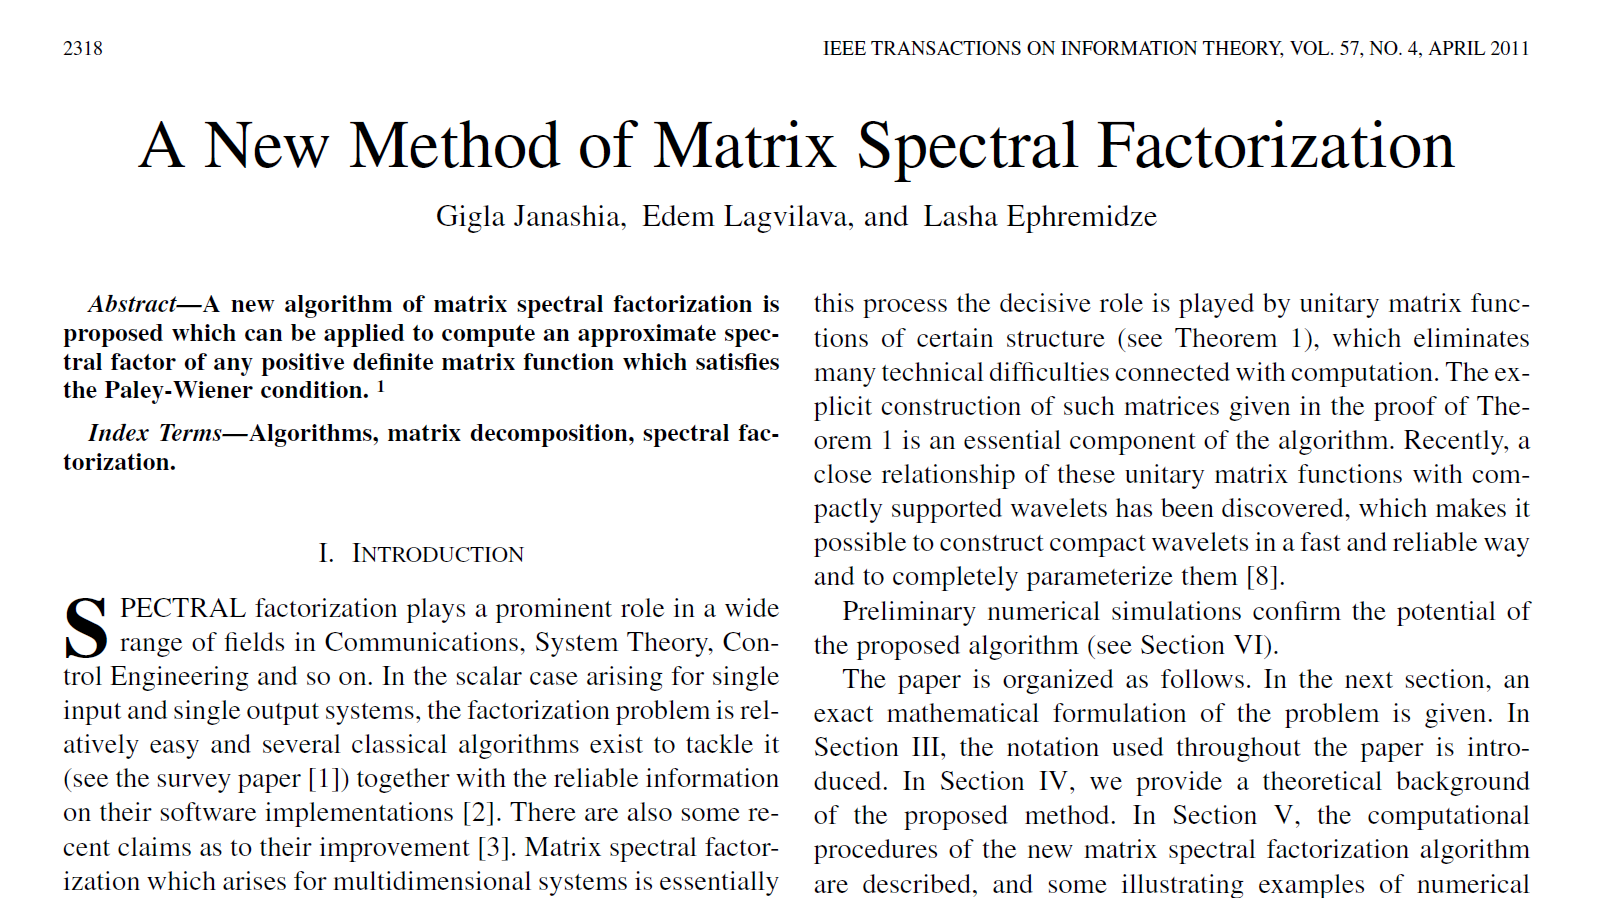
\includegraphics[scale=.35]{fig/ANewMethod.png}
\end{frame}




%%%%%%%%%%%%%%%%%%%%%%%%%%%%%%%%%%%%%%%%%%%%%%%%%%%%%%%%%%%%%%%%%%%%%%%%%%%%%%%%%%%%%%%
%%%%%%%%%%%%%%%%%%%%%%%%%%%%%%%%%%%%%%%%%%%%%%%%%%%%%%%%%%%%%%%%%%%%%%%%%%%%%%%%%%%%%%%
\section{The Wiener Projection}
%%%%%%%%%%%%%%%%%%%%%%%%%%%%%%%%%%%%%%%%%%%%%%%%%%%%%%%%%%%%%%%%%%%%%%%%%%%%%%%%%%%%%%%

\begin{frame}{This Approach}
Given a full model
$$X_n = F(X_n)$$
with resolved variables collected in $x_n$,
select functions $\psi^{(i)}(x)$ (informed by model) on reduced state variables.
$$\psi(x) = \Big(\psi^{(0)}(x)\Big|\psi^{(1)}(x)\Big|\cdots\Big|\psi^{(\nu)}\Big)
\qquad\text{and}\qquad\psi_k = \psi(x_k).$$
The reduced model we purpose is of the form,

\begin{equation*}
\boxed{x_{n+1} =  \sum_{k=0}^\infty \psi_{k}\cdot h_{n-k} + \xi_{n+1}}
\end{equation*}
We use the data to infer $h_{k}$ and $\xi_{n}$ (described briefly below).

\end{frame}

%%%%%%%%%%%%%%%%%%%%%%%%%%%%%%%%%%%%%%%%%%%%%%%%%%%%%%%%%%%%%%%%%%%%%%%%%%%%%%%%%%%%%%%

\begin{frame}{How to solve}
	Dr. Kevin Lin and Dr. Fei Lu solves in time domain, using an iterative optimization algorithm. 
	
	\bigskip
	
	This study investigates computing the Wiener filter by spectral methods (that is, employing information like the power spectra $S_{yx}$ and $S_{x}$).  This is a direct method requiring no iterative optimization
	
	\bigskip
	
	Advantages:
	\begin{itemize}
		\item Quicker
		\item more accurate (?)
	\end{itemize}
\end{frame}


%%%%%%%%%%%%%%%%%%%%%%%%%%%%%%%%%%%%%%%%%%%%%%%%%%%%%%%%%%%%%%%%%%%%%%%%%%%%%%%%%%%%%%%
\section{Numerical Impimentation: Programing the Wiener-Hopf Technique}
%%%%%%%%%%%%%%%%%%%%%%%%%%%%%%%%%%%%%%%%%%%%%%%%%%%%%%%%%%%%%%%%%%%%%%%%%%%%%%%%%%%%%%%

%%%%%%%%%%%%%%%%%%%%%%%%%%%%%%%%%%%%%%%%%%%%%%%%%%%%%%%%%%%%%%%%%%%%%%%%%%%%%%%%%%%%%%%
\section{Examples}
%%%%%%%%%%%%%%%%%%%%%%%%%%%%%%%%%%%%%%%%%%%%%%%%%%%%%%%%%%%%%%%%%%%%%%%%%%%%%%%%%%%%%%%
\begin{frame}{Example 1: MA(1) Signal, Additive WN}
	Let $\textbf{y} \sim \text{MA}(1)$ with $r \in \R$ have the form 
	$$\textbf{y}_n = \textbf{u}_n - r\textbf{u}_{n-1} \qquad \text{for } n > -\infty$$
	$\textbf{u}_n \sim N(0,1)$ i.i.d. And let $y_n$ be a realization, this will be the signal. The observations are
	$$x_n = y_n + v_n, \qquad \text{for } n > -\infty.$$
	we assume $\textbf{v}_n \sim N(0,\sigma_{\textbf{v}})$ i.i.d.  and are uncorrelated with $\textbf{y}$. 
	
	\bigskip
	
	To compute the Wiener filter we need $S_{\textbf{yx}}$, $S^+_{\textbf{x}}$, and $S^-_{\textbf{x}}$.
	First, observe
	$$S_{\textbf{yx}} = S_{\textbf{y}} + S_{\textbf{yv}} = S_{\textbf{y}},$$
	and 
	$$S_{\textbf{x}} = S_{\textbf{y}+\textbf{v},\textbf{y}+\textbf{v}} = S_{\textbf{y}} + S_{\textbf{yv}} + S_{\textbf{vy}} + S_{\textbf{v}} = S_{\textbf{y}} + \sigma_{\textbf{v}}^2.$$ 
\end{frame}	

%%%%%%%%%%%%%%%%%%%%%%%%%%%%%%%%%%%%%%%%%%%%%%%%%%%%%%%%%%%%%%%%%%%%%%%%%%%%%%%%%%%%%%%

\begin{frame}{Example 1: MA(1) Signal, Additive WN}
	(Just this once we compute it for clarity)
	\begin{align*}
	S_{\textbf{y}} &= \sum_{k = -\infty}^\infty \E[(u_{n+k} - ru_{n+k-1})(u_n - ru_{n-1})^*]z^{-k} \\
	&= \sum_{k = -\infty}^\infty \E[u_{n+k}u^*_n - ru_{n+k-1}u^*_n - ru_{n+k}u^*_{n-1} + r^2u_{n+k-1}u^*_{n-1}]z^{-k} \\
	&= \sum_{k = -\infty}^\infty \big(\delta(k) - r\delta(k-1) - r\delta(k+1) +r^2\delta(k)\big)z^{-k} \\
	&= 1 + r^2 - rz^{-1} - rz \qquad \big(\quad = (1-rz)(1-rz^{-1})\quad\big).
	\end{align*}
	So, $S_{\textbf{yx}}(z) = (1-rz)(1-rz^{-1})$ and
	\begin{align*}
	S_{\textbf{x}}(z) &= 1 + r^2 + \sigma_{\textbf{v}}^2 - rz^{-1} - rz\\
	& = \frac{r}{\rho}(1 - \rho z^{-1})(1 - \rho z)
	\end{align*}
	For a suitably chosen $\rho$, $|\rho| < 1$.
\end{frame}	

%%%%%%%%%%%%%%%%%%%%%%%%%%%%%%%%%%%%%%%%%%%%%%%%%%%%%%%%%%%%%%%%%%%%%%%%%%%%%%%%%%%%%%%

\begin{frame}{Example 1: MA(1) Signal, Additive WN}
	For  $S^+_{\textbf{x}}$ and $S^-_{\textbf{x}}$ we then get
	$$S^+_{\textbf{x}}(z) = \sqrt{\frac{r}{\rho}}  (1-\rho z) \and S^-_{\textbf{x}}(z) = \sqrt{\frac{r}{\rho}}  (1-\rho z^{-1}).$$
	Putting this together we get
	\begin{align*}
	\frac{S_{\textbf{yx}}(z)}{S^+_{\textbf{x}}(z)}&= \frac{1 + r^2 -rz^{-1} - rz }{\sqrt{\frac{r}{\rho}}  (1-\rho z)}\\
	&= \sqrt{\frac{\rho}{r}}(1 + r^2 -rz^{-1} - rz)\sum_{n=0}^\infty (\rho z)^n\\
	&= -\sqrt{\rho r}z^{-1} +\sqrt{\frac{\rho}{r}}(1+r^2) - \rho \sqrt{\rho r} + \sum_{n=1}^\infty  \xi_n z^n.
	\end{align*}
	Which means
	$$
	\left\{\frac{S_{\textbf{yx}}(z)}{S^+_{\textbf{x}}(z)}\right\}_+ =-\sqrt{\rho r}z^{-1} +\sqrt{\frac{\rho}{r}}(1+r^2) - \rho \sqrt{\rho r}.$$
	
\end{frame}	

%%%%%%%%%%%%%%%%%%%%%%%%%%%%%%%%%%%%%%%%%%%%%%%%%%%%%%%%%%%%%%%%%%%%%%%%%%%%%%%%%%%%%%%

\begin{frame}{Example 1: MA(1) Signal, Additive WN}
	\begin{align*}
	H(z) = \frac{1}{S^-_{\textbf{x}}(z)} \left\{\frac{S_{\textbf{yx}(z)}}{S^+_{\textbf{x}}(z)}\right\}_+ &= \frac{1}{\sqrt{\frac{r}{\rho}}  (1-\rho z^{-1})}\left( \sqrt{\rho r}z^{-1} +\sqrt{\frac{\rho}{r}}(1+r^2) - \rho \sqrt{\rho r}\right) \\
	&= \left[\frac{1+r^2}{r}\rho - \rho^2\right] + \sum_{n=1}^\infty \rho^n \left[\frac{1+r^2}{r}\rho - \rho^2 - 1\right]z^{-n}
	\end{align*}
	If we let $d = \dfrac{1+r^2}{r}\rho - \rho^2 $, then
	$$H(z) = d + \sum_{n=1}^\infty \rho^n (d-1)z^{-n}$$
	And the causal filter $h = (h_n, n > -\infty)$ is 
	\begin{center}
		\begin{tabular}{l @{\qquad} r}
			$ h_n = 0 $ & if $n<0$ \\
			$ h_n = d $ & if $n=0$ \\
			$ h_n = \rho^n(d-1) $ & if $n>0$
		\end{tabular}
	\end{center}
\end{frame}

%%%%%%%%%%%%%%%%%%%%%%%%%%%%%%%%%%%%%%%%%%%%%%%%%%%%%%%%%%%%%%%%%%%%%%%%%%%%%%%%%%%%%%%

\begin{frame}{Example 1: MA(1) Signal, Additive WN}
	Here is a run, with $r=10$, $\sigma_{\textbf{v}} = 10$. The trajectory has $10^6$ steps after discarding $10^3$ steps. 
	
	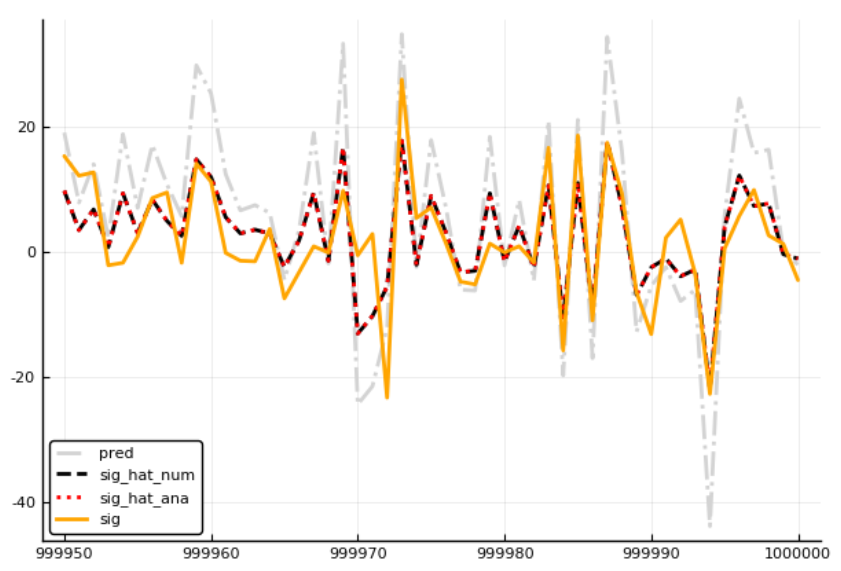
\includegraphics[scale=.33]{fig/figMA1_ts.png}
	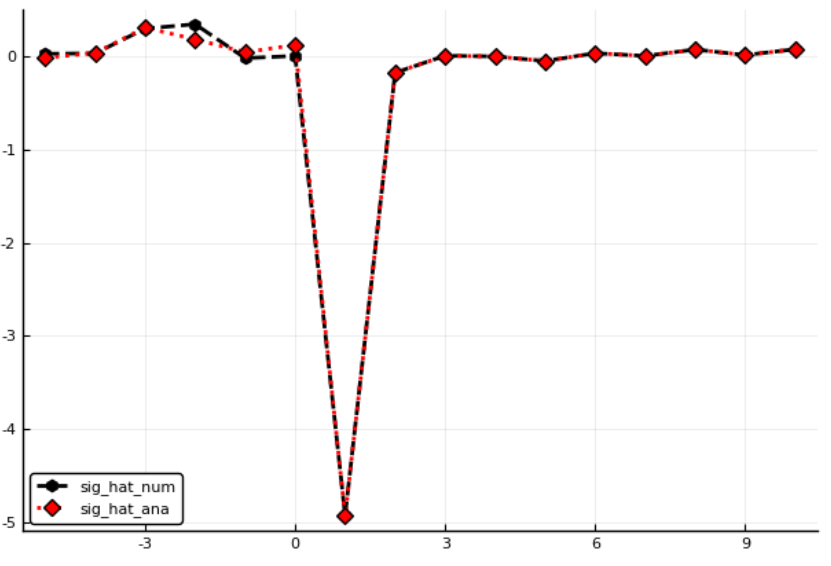
\includegraphics[scale=.33]{fig/figMA1_cov.png}
	
	Left: A window of the time series for the signal (orange), the predictors (light gray), the estimated signal using the analytic and numerical Wiener filter (red, black). 
	
	Right: The covariance between errors (red from analytic filter, black from numerical) and predictors (observations). \\
\end{frame}


%%%%%%%%%%%%%%%%%%%%%%%%%%%%%%%%%%%%%%%%%%%%%%%%%%%%%%%%%%%%%%%%%%%%%%%%%%%%%%%%%%%%%%%
%%%%%%%%%%%%%%%%%%%%%%%%%%%%%%%%%%%%%%%%%%%%%%%%%%%%%%%%%%%%%%%%%%%%%%%%%%%%%%%%%%%%%%%


\begin{frame}{Example 2: MA(2) Signal, Additive WN}
	For the signal in this example we use the MA(2) process,
	$$y_n = u_n + r_1u_{n-1} + r_2u_{n-2}, \qquad \text{for } n > -\infty$$
	where $r_1,r_2\in \R$.  The observations will again simply be the signal with an additive white noise,
	$$x_n = y_n + v_n, \qquad \text{for } n > -\infty.$$
	We assume that $\textbf{v} = (\textbf{v}_n ,  n > -\infty)$ is uncorrelated with $\textbf{y}$. 
	
	
	\bigskip
	
	Skipping ahead we have 
	$$S_{\textbf{yx}} = 1 + r_1^2 + r_2^2 + (r_1 + r_1r_2)(z + z^{-1}) + r_2(z^2 + z^{-2}),$$
	$$S^+_{\textbf{x}}(z) = \sqrt{\frac{r_2}{\rho_1\rho_2}}  (1-\rho_1 z)(1-\rho_2 z)\quad\text{and}\quad S^-_{\textbf{x}}(z) = \sqrt{\frac{r_2}{\rho_1\rho_2}}  (1-\rho_1 z^{-1})(1-\rho_2 z^{-1}).$$
	
\end{frame}	

%%%%%%%%%%%%%%%%%%%%%%%%%%%%%%%%%%%%%%%%%%%%%%%%%%%%%%%%%%%%%%%%%%%%%%%%%%%%%%%%%%%%%%%

\begin{frame}{Example 2: MA(2) Signal, Additive WN}
	\vspace{-.7cm}\begin{align*}
	H(z) &= \frac{1}{S^-_{\textbf{x}}(z)} \left\{\frac{S_{\textbf{yx}}(z)}{S^+_{\textbf{x}}(z)}\right\}_+ = \frac{\sqrt{\frac{r_2}{\rho_1\rho_2}}(\alpha_2 z^{-2} + \alpha_1 z^{-1} + \alpha_0)}{\sqrt{\frac{r_2}{\rho_1\rho_2}}  (1-\rho_1 z^{-1})(1-\rho_2 z^{-1})}\\
	& = (\alpha_2 z^{-2} + \alpha_1 z^{-1} + \alpha_0)\left(\sum_{n=0}^\infty \rho_1^nz^{-n}\right)
	\left(\sum_{m=0}^\infty \rho_2^mz^{-m}\right)\\
	&=  \alpha_0\alpha(0) + [\alpha_0\alpha(1) + \alpha_1\alpha(0)]z^{-1} \\
		&\qquad + \sum_{n=2}^\infty [\alpha_0\alpha(n)+\alpha_1\alpha(n-1)+\alpha_2\alpha(n-2)]z^{-n}
	\end{align*}
	where
	$\alpha(n) = \displaystyle \sum_{k=0}^n \rho_1^{n-k}\rho_2^k $\quad
	and 
	\begin{align*}
	\alpha_0 &= \frac{\rho_1\rho_2}{r_2}\big[r_2(\rho_1^2 + \rho_2^2 + \rho_1\rho_2) + (r_1 + r_1r_2)(\rho_1 + \rho_2) + 1 + r_1^2  + r_2^2\big],\\
	\alpha_1 &=  \frac{\rho_1\rho_2}{r_2}\big[r_2(\rho_1+\rho_2) + r_1 +r_1 r_2\big],\qquad  \alpha_2 = \frac{\rho_1\rho_2}{r_2}r_2.
	\end{align*}
\end{frame}	

%%%%%%%%%%%%%%%%%%%%%%%%%%%%%%%%%%%%%%%%%%%%%%%%%%%%%%%%%%%%%%%%%%%%%%%%%%%%%%%%%%%%%%%

\begin{frame}{Example 2: MA(2) Signal, Additive WN}
	And the causal filter $h = (h_n, n > -\infty)$ is 
	\begin{center}
		\bigskip
		\begin{tabular}{l @{\qquad} r}
			$ h_n = 0 $ & if $n<0$ \\
			$ h_n = \alpha_0\alpha(0) $ & if $n=0$ \\
			$ h_n = \alpha_0\alpha(1) + \alpha_1\alpha(0) $ & if $n=1$ \\
			$ h_n = \alpha_0\alpha(n)+\alpha_1\alpha(n-1)+\alpha_2\alpha(n-2) $ & if $n\ge2$
		\end{tabular}
	\end{center}
\end{frame}	

%%%%%%%%%%%%%%%%%%%%%%%%%%%%%%%%%%%%%%%%%%%%%%%%%%%%%%%%%%%%%%%%%%%%%%%%%%%%%%%%%%%%%%%

\begin{frame}{Example 2: MA(2) Signal, Additive WN}
	Here is a run, with $r=10$, $\sigma_{\textbf{v}} = 10$. The trajectory has $10^6$ steps after discarding $10^3$ steps. 
	
	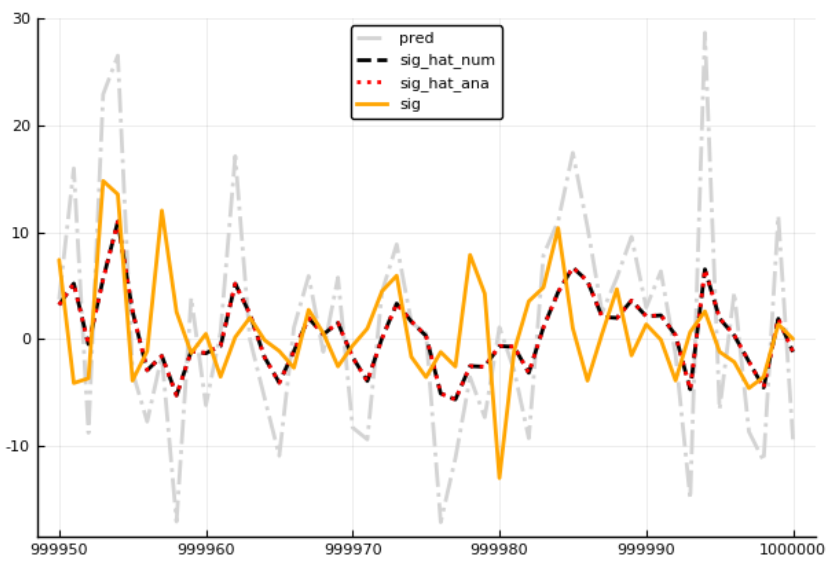
\includegraphics[scale=.33]{fig/figMA2_ts.png}
	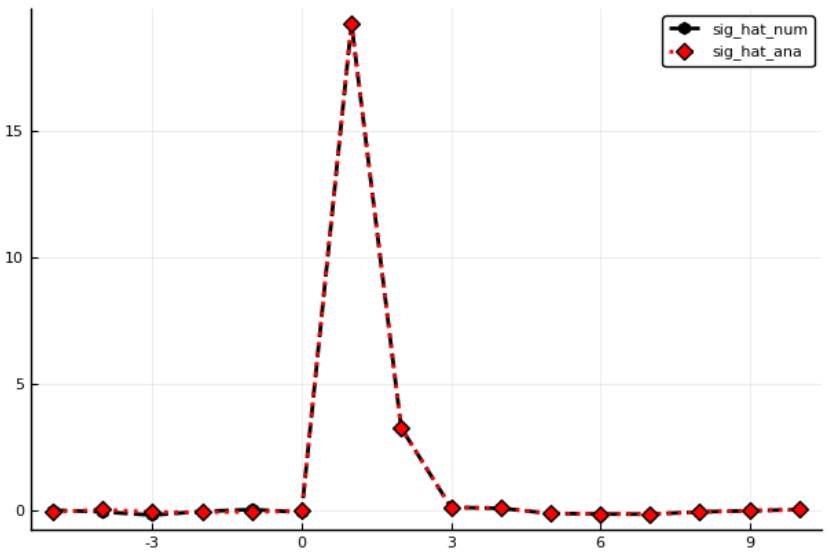
\includegraphics[scale=.33]{fig/figMA2_cov.png}
	
	Left: A window of the time series for the signal (orange), the predictors (light gray), the estimated signal using the analytic and numerical Wiener filter (red, black). 
	
	Right: The covariance between errors (red from analytic filter, black from numerical) and predictors (observations). \\
\end{frame}


%%%%%%%%%%%%%%%%%%%%%%%%%%%%%%%%%%%%%%%%%%%%%%%%%%%%%%%%%%%%%%%%%%%%%%%%%%%%%%%%%%%%%%%
%%%%%%%%%%%%%%%%%%%%%%%%%%%%%%%%%%%%%%%%%%%%%%%%%%%%%%%%%%%%%%%%%%%%%%%%%%%%%%%%%%%%%%%


\begin{frame}{Example 3: AR(2) Signal, Additive WN}
	Let us consider the stationary autoregressive process of order 2,
	$$y_n = (r_1+r_2)y_{n-1} - r_1r_2 y_{n-2} + u_n , \qquad \text{for } n > -\infty$$
	for $r_1,r_2 \in \{z : |z|<1\}$.
	
	
	\bigskip
	
	Skipping way ahead we have 
	\begin{align*}
	S_{\textbf{yx}} &= \frac{1}{ (1 - r_1z^{-1})(1 - r_2z^{-1})(1 - r_1^*z)(1 - r_2^*z)},\\
	S^+_{\textbf{x}}(z) &= \sqrt{\sigma_{\textbf{v}}^2\frac{r^*_1r^*_2}{\rho_1^*\rho_2^*}} \frac{(1 - \rho_1^*z)(1 - \rho_2^*z)}{(1 - r_1^*z)(1 - r_2^*z)},\\
	S^-_{\textbf{x}}(z) &= \sqrt{\sigma_{\textbf{v}}^2\frac{r^*_1r^*_2}{\rho_1^*\rho_2^*}} \frac{(1 - \rho_1z^{-1})(1 - \rho_2z^{-1})}{(1 - r_1z^{-1})(1 - r_2z^{-1})}.
	\end{align*}$$
	$$
	
\end{frame}	

%%%%%%%%%%%%%%%%%%%%%%%%%%%%%%%%%%%%%%%%%%%%%%%%%%%%%%%%%%%%%%%%%%%%%%%%%%%%%%%%%%%%%%%

\begin{frame}{Example 3: AR(2) Signal, Additive WN}
	And the causal filter $h = (h_n, n > -\infty)$ is 
	\begin{center}
		\bigskip
		\begin{tabular}{l @{\qquad} r}
			$ h_n = 0 $ & if $n<0$ \\
			$ h_n = \phi(0) $ & if $n=0$ \\
			$ h_n = \phi(1) - \phi(0)(r_1+r_2) $ & if $n=1$ \\
			$ h_n = \phi(n) - (r_1+r_2)\phi(n-1) + r_1r_2 \phi(n-2) $ & if $n\ge2$
		\end{tabular}
	\end{center}
Where $$\phi(n) = \phi_0^2 \sum_{k=0}^n \gamma(n-k)\alpha(k),\qquad \alpha(n) = \sum_{k=0}^n \rho_1^{n-k}\rho_2^k,\qquad\beta(n) = \sum_{k=0}^n r_1^{n-k}r_2^k,$$
and $$\gamma(n) = 
\begin{cases}
\displaystyle \sum_{k=0}^\infty \alpha^*(k-n)\beta(k) & n\le 0\\
\displaystyle \sum_{k=0}^\infty \alpha^*(k)\beta(k+n) & n > 0
\end{cases}$$
\end{frame}	

%%%%%%%%%%%%%%%%%%%%%%%%%%%%%%%%%%%%%%%%%%%%%%%%%%%%%%%%%%%%%%%%%%%%%%%%%%%%%%%%%%%%%%%

\begin{frame}{Example 3: AR(2)) Signal, Additive WN}
	Here is a run, with $r1, r2 = .5, .95$, $\sigma_{\textbf{v}} = 4$. The trajectory has $10^6$ steps after discarding $10^3$ steps. 
	
	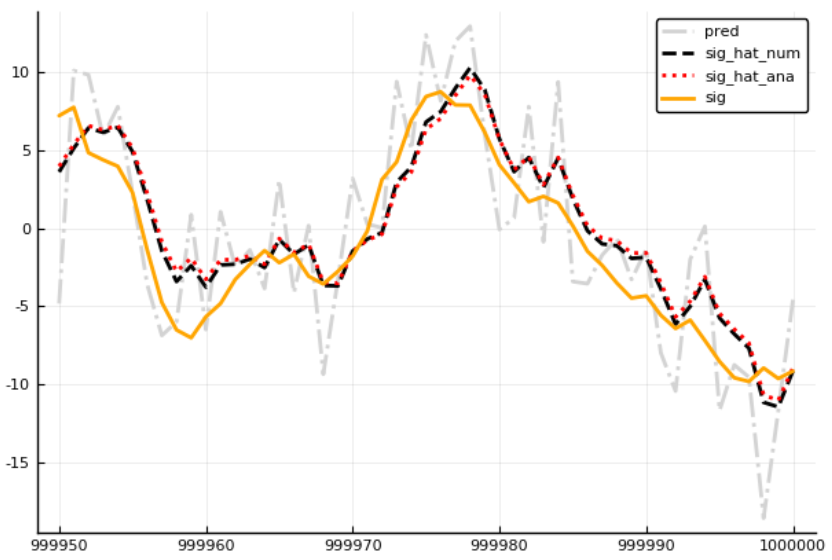
\includegraphics[scale=.33]{fig/figAR2_ts.png}
	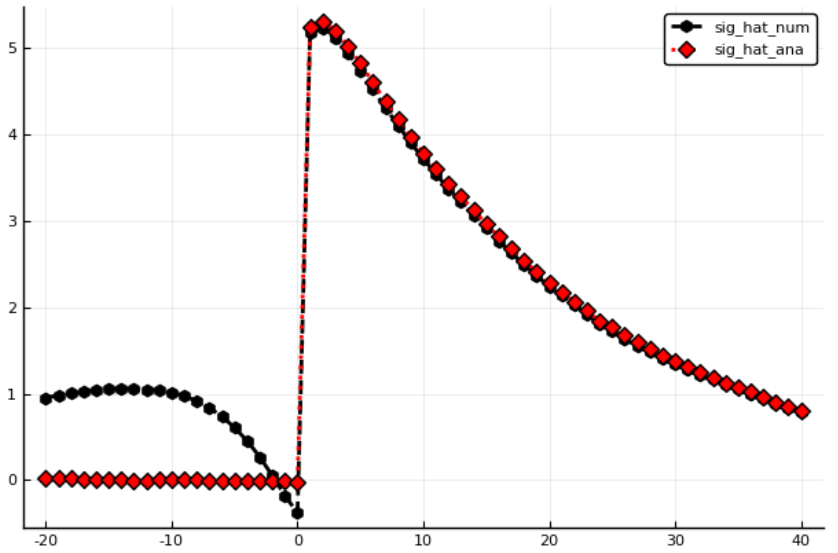
\includegraphics[scale=.33]{fig/figAR2_cov.png}
	
	Left: A window of the time series for the signal (orange), the predictors (light gray), the estimated signal using the analytic and numerical Wiener filter (red, black). 
	
	Right: The covariance between errors (red from analytic filter, black from numerical) and predictors (observations). \\
\end{frame}


%%%%%%%%%%%%%%%%%%%%%%%%%%%%%%%%%%%%%%%%%%%%%%%%%%%%%%%%%%%%%%%%%%%%%%%%%%%%%%%%%%%%%%%
%%%%%%%%%%%%%%%%%%%%%%%%%%%%%%%%%%%%%%%%%%%%%%%%%%%%%%%%%%%%%%%%%%%%%%%%%%%%%%%%%%%%%%%

\begin{frame}{Example 4: AR(2) Signal, Filtered, Ad. WN}
	Let us consider again the stationary autoregressive process of order 2,
	$$y_n = (r_1+r_2)y_{n-1} - r_1r_2 y_{n-2} + u_n , \qquad \text{for } n > -\infty$$
	for $r_1,r_2 \in \{z : |z|<1\}$.
	This time however, we define the observations to be the signal $y$ operated upon by a finite impulse response time invariant filter $w$ with additive white noise.
	$$x_n = (w * y)_n + v_n, \qquad \text{for } n > -\infty.$$
	
	For simplicity let $$ w = (\dots,0,\fbox{1},w_1, w_2,0,\dots),$$
	where the box indicate the element indexed by 0 and $w_1,w_2 \in \R$, then write
	$$W(z) = \sum_{k = -\infty}^\infty w_k z^{-k} = 1 + w_1 z^{-1} + w_2 z^{-2}.$$
	
\end{frame}	


%%%%%%%%%%%%%%%%%%%%%%%%%%%%%%%%%%%%%%%%%%%%%%%%%%%%%%%%%%%%%%%%%%%%%%%%%%%%%%%%%%%%%%%


\begin{frame}{Example 4: AR(2) Signal, Filtered, Ad. WN}
Observe that 
$$S_{\textbf{yx}}(z) = S_{\textbf{y}}(z)W^*(z^{-*}) \and S_{\textbf{x}} = W(z)S_{\textbf{y}}(z)W^*(z^{-*}) + \sigma_{\textbf{v}}^2.$$
So, 
\begin{align*}
S_{\textbf{yx}}(z) &= \frac{1 + w_1 z + w_2 z^{2}}{ (1 - r_1z^{-1})(1 - r_2z^{-1})(1 - r_1^*z)(1 - r_2^*z)}\\
\end{align*}
and
\begin{align*}
S_{\textbf{x}}(z) &=\frac{w_2 + \sigma_{\textbf{v}}^2r^*_1r^*_2}{\rho_1^*\rho_2^*}\cdot \frac{(1 - \rho_1z^{-1})(1 - \rho_2z^{-1})(1 - \rho_1^*z)(1 - \rho_2^*z)}{(1 - r_1z^{-1})(1 - r_2z^{-1})(1 - r_1^*z)(1 - r_2^*z)}
\end{align*} 
For suitable $\rho_1,\rho_2$ (which depend on $w_1,w_2$) 
\end{frame}	

%%%%%%%%%%%%%%%%%%%%%%%%%%%%%%%%%%%%%%%%%%%%%%%%%%%%%%%%%%%%%%%%%%%%%%%%%%%%%%%%%%%%%%%

\begin{frame}{Example 4: AR(2) Signal, Filtered, Ad. WN}
So, the causal filter $h = (h_n, n > -\infty)$ is 
\begin{center}
	\bigskip
	\begin{tabular}{l @{\qquad} r}
		$ h_n = 0 $ & if $n<0$ \\
		$ h_n = \psi(0) $ & if $n=0$ \\
		$ h_n = \psi(1) - \psi(0)(r_1+r_2) $ & if $n=1$ \\
		$ h_n = \psi(n) - (r_1+r_2)\psi(n-1) + r_1r_2 \psi(n-2) $ & if $n\ge2$
	\end{tabular}
\end{center}
	Where $$\psi(n) = \psi_0^2 \sum_{k=0}^n \big[\gamma(n-k) + w_1\gamma(n-k+1) + w_2\gamma(n-k+2)\big]\alpha(k).$$
\end{frame}	

%%%%%%%%%%%%%%%%%%%%%%%%%%%%%%%%%%%%%%%%%%%%%%%%%%%%%%%%%%%%%%%%%%%%%%%%%%%%%%%%%%%%%%%

\begin{frame}{Example 4: AR(2) Signal, Filtered, Ad. WN}
	Here is a run, with $r_1,r_2 = -0.2, 0.9$, $w_1,w_2 = -0.1, 5$, and $\sigma_{\textbf{v}} = 1.1$. The trajectory has $10^6$ steps after discarding $10^3$ steps. 
	
	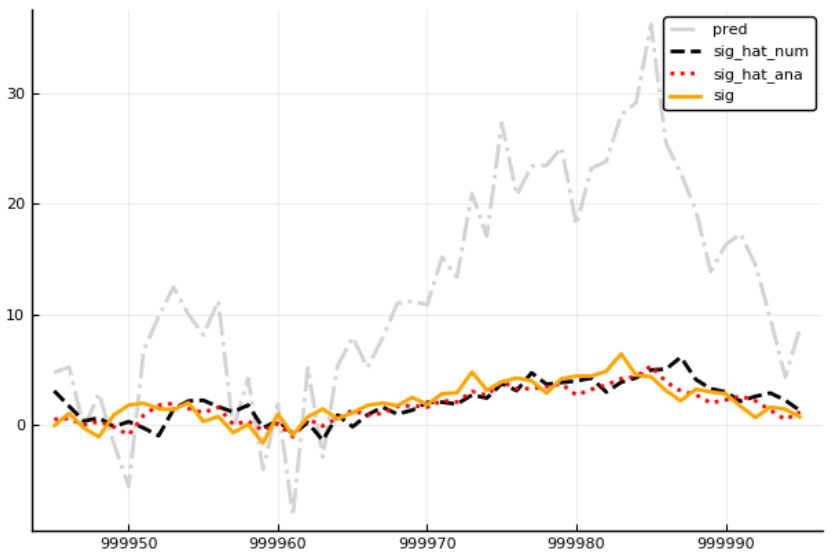
\includegraphics[scale=.33]{fig/figAR2F_ts.png}
	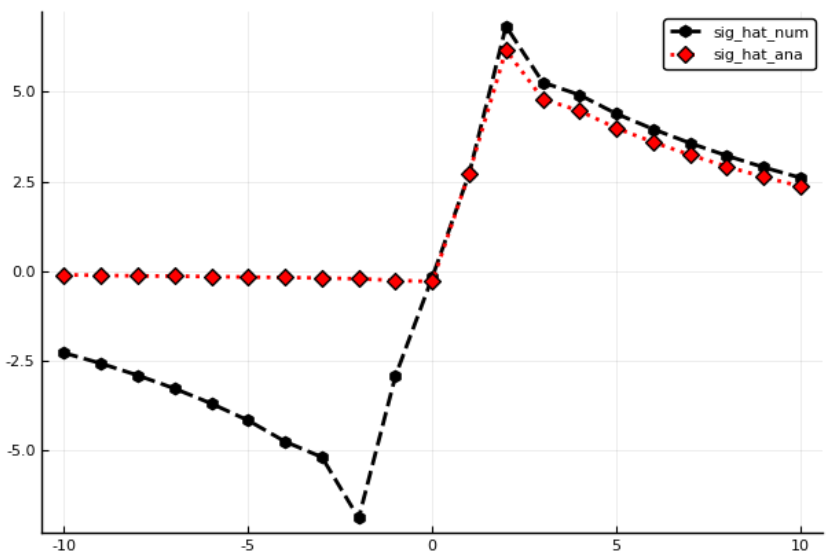
\includegraphics[scale=.33]{fig/figAR2F_cov.png}
	
	Left: A window of the time series for the signal (orange), the predictors (light gray), the estimated signal using the analytic and numerical Wiener filter (red, black). 
	
	Right: The covariance between errors (red from analytic filter, black from numerical) and predictors (observations). \\
\end{frame}


%%%%%%%%%%%%%%%%%%%%%%%%%%%%%%%%%%%%%%%%%%%%%%%%%%%%%%%%%%%%%%%%%%%%%%%%%%%%%%%%%%%%%%%
%%%%%%%%%%%%%%%%%%%%%%%%%%%%%%%%%%%%%%%%%%%%%%%%%%%%%%%%%%%%%%%%%%%%%%%%%%%%%%%%%%%%%%%
\section{Conclusions}
%%%%%%%%%%%%%%%%%%%%%%%%%%%%%%%%%%%%%%%%%%%%%%%%%%%%%%%%%%%%%%%%%%%%%%%%%%%%%%%%%%%%%%%



\begin{frame}
Thank you!
\end{frame}


\end{document}




